\section{Motivation}
\subsection{Physic settings}
For the psychics we had to set two important setting, that are most important for computing whether the bridge will crash or not. These are the mass of the train and the strength of the breaking points. For both we tested 3 different settings, so in total we tested 9 combinations. The test was building 3 bridges that are shown in figure X. The first two should fail and the last bridge should pass. \\
\begin{figure}[H]
    \centering
    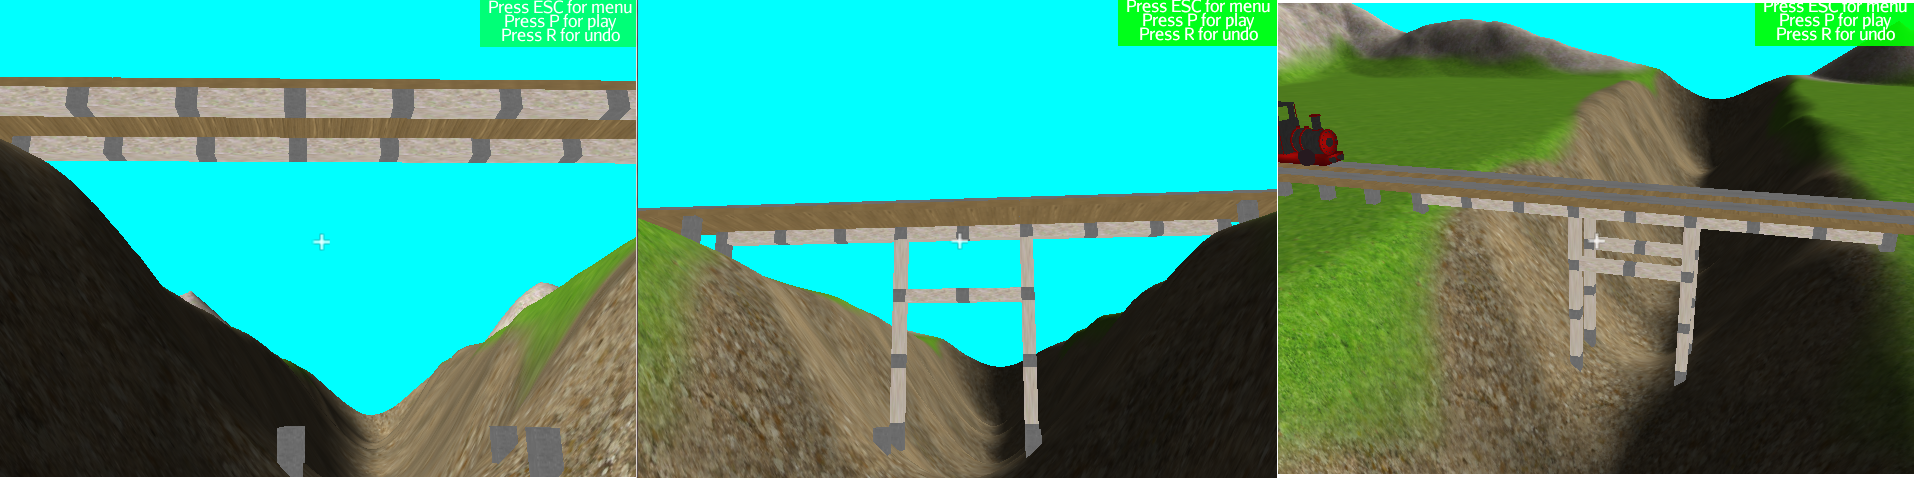
\includegraphics[width=1.0\textwidth]{screenshots/bridges.png}
    \caption{The three test bridges}
    \label{fig:bridges}
\end{figure}
So the correct order in each cell should be FFS. (Where the F is fail, S is success and E is strange behaviour). \\
\begin{figure}[H]
    \centering
    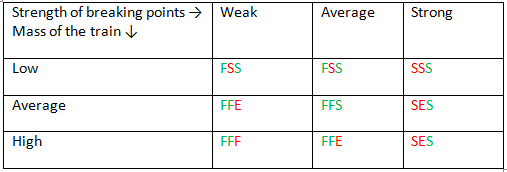
\includegraphics[width=0.8\textwidth]{screenshots/table.png}
    \caption{The results of the tests}
    \label{fig:table}
\end{figure}
Before we started with testing, we only thought it would fail or succeed, but during testing we had to add another option. The E for strange behaviour. During some of the tests, the simulation of the train over the bridge became very unrealistic and thus we could not really call it a succes. \\
It is not really a suprise, that both average mass and average strenght of the connections gives the best results. We first builded a few bridges and changed the mass of the train and the strenght of the connections to make them more realistic. We did this test afterwards to test if there are no better combinations. \\